\section{Numerical Experiments}\label{sec:exp}
The experiments were carried out on \angus{insert details of machine and OS here}. All code was implemented and executed in MATLAB\angus{version number}, with kriging and co-kriging models constructed using the ooDACE toolbox.

The \AlgName{} algorithm was compared against a baseline co-kriging algorithm and an implementation of the \motos{}~\cite{xu2016mo2tos}. All algorithms were run 30 times on each problem instance for the equivalent of 2000 low-fidelity evaluations, recording the best objective value, the mean and standard deviation of the resulting solutions produced by each trial.

To establish statistical significance of the results, a pairwise comparison was made using the Mann-Whitney-Wilcoxon (MWW) test~\cite{mann1947test}, with the number of ``wins'', ``losses'' and ``draws'' recorded for each algorithm. For each pairwise comparison, let $\delta^p_{ab} = \mu^p_a - \mu^p_b$, with $\mu^p_i$ being the mean objective value for algorithm $i$ on problem instance $p$ over all trials. If the $p$-value for MWW is less than 0.05 and $|\delta^p_{ab}| > 10^{-5}$, algorithm $a$ is said to have ``won'' when $\delta^p_{ab} < 0$, ``lost'' when $\delta^p_{ab} > 0$ and ``drawn'' if both initial conditions are not met.

\subsection{Datasets}
The experiments were run on a collection of bound-constrained, single-objective, multi-fidelity test functions that can be divided into two different datasets. The first set (dataset $A$) is a selection of problem instances taken from Lv~et~al.~\cite{lv2021multi}. Problems $f10$ to $f17$ were chosen from this dataset as they contain between three and eight decision variables, determined as a representative range of easy to difficult problems. The explicit definitions for both the high- and low-fidelity functions are provided in the Appendix.

The second set of problem instances (dataset $B$) is generated using the well-known Griewank~\cite{griewank1981generalized} and Michalewicz~\cite{michalewicz2013genetic} test problems (Figures~\ref{fig:grie} and~\ref{fig:michal})\hemant{To be consistent, we can include the problem definitions instead of figures for these problems as well. Figures 5 and 6 can therefore be removed}. Each problem was instantiated with versions for three, five and eight decision variables. This matches the range of the first dataset, and also allows the performance of the algorithms to be judged across different sized problems in a more controlled environment. These test problems are not naturally multi-fidelity optimisation problems, so low-fidelity evaluations are constructed by applying the methods described in~\cite{wang2017generic}. Two different error functions were tested for each instance, modelling two types of fidelity error: resolution and stochastic. An appropriate fidelity level $\phi$ for each problem was chosen by computing the square of the Pearson correlation coefficient $r^2$ for different fidelity values and selecting a value for $\phi$ such that $r^2$ was between 0.65 and 0.85, to be commensurate with the first dataset.

See Tables~\ref{tab:funcs} and~\ref{tab:errfuncs} in Appendix~\ref{app:testfuncs} for test function and error function equations, respectively.

\begin{figure}[h!]
  \centering
  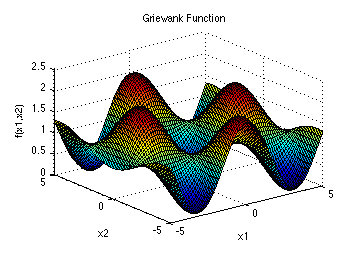
\includegraphics[width = 0.40\textwidth]{img/griewank.png} 
  \caption{The Griewank test function in 2D.\angus{will do a better version}} 
    \label{fig:grie}
\end{figure}
\begin{figure}[h!]
  \centering
  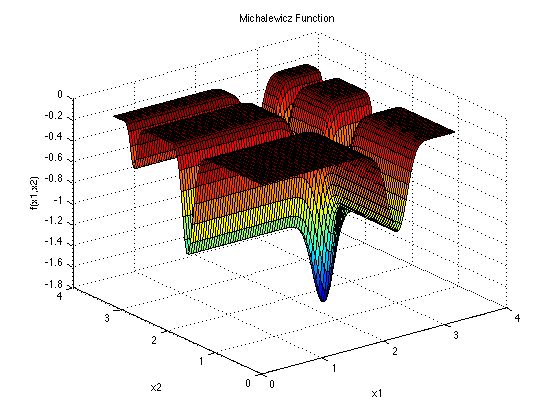
\includegraphics[width = 0.40\textwidth]{img/michal.png} 
  \caption{The Michalewicz test function in 2D.\angus{will do a better version}} 
    \label{fig:michal}
\end{figure}

\subsection{\AlgName{} parameters}
The \AlgName{} algorithm can be viewed as a modular framework within which various search and modeling methods can be implemented. Therefore, its components can be divided into two categories: \AlgName{} specific components, which are intrinsic to its operation and whose parameters are also intrinsic; and, generic method components, such as global search techniques and modelling methods which can be substituted for other similar techniques, which come with their own parameters. The \AlgName{} specific parameters are discussed in general in Section~\ref{sec:method}; this section will detail the specific values for these  parameters and for the generic search method used.

To reduce the number of arbitrary parameters, initial population sizes are defined as a function of problem size. The high-fidelity population has a size of $6D$, as this is the smallest number of high-fidelity solutions that can be used to generate a co-kriging model for all of the instances, with the low-fidelity population being $18D$, which was chosen using sensitivity analysis to find the smallest value which still produces good solutions across the whole set of instances.

The maximum size that the low-fidelity archive can reach before it must be truncated is 400, this was chosen because values much higher than this significantly slow the procedure down while yielding minimal-to-no improvment. 

In the $LocalOCBA$ procedure, the total number of solutions to be sampled, $\Delta_1$, is 25 and the number of samples per statistics update, $\Delta_2$, is 5. These were chosen to provide a good balance between speed and efficiency. The clustering method used to partition the solutions is $k$-means clustering, with the value for $k$ being chosen using the so-called \emph{elbow method}\hemant{Any references for this method?}.

Differential evolution (DE)~\cite{storn1997differential} was used to globally search the updated co-kriging model. This DE was run over 30 generations with a crossover rate of 0.9, a mutation factor of 0.5 and a population size of 100. \hemant{Mention the type of operators used (they have identifiers such as rand/bin etc.}

The kriging models used are from the ooDACE toolbox~\cite{oodace}, with the default paramters.

\subsection{Baseline co-kriging algorithm}
Co-kriging is a popular approach to solving many multi-fidelity problems. The outer-loop of the \AlgName{} algorithm functions by iteratively updating a co-kriging model using data from a modified version of the OCBA procedure. In order to demonstrate the effectiveness of this new technique, the performance of \AlgName{} is compared against the baseline simple co-kriging algorithm given in Algorithm~\ref{alg:co-kriging}.


\begin{algorithm}[h!] 
\caption{Baseline co-kriging procedure}
\label{alg:co-kriging}
\algsetup{linenosize=\footnotesize}
{\footnotesize
\begin{algorithmic}[1]
\REQUIRE{$P$, problem data; $N_{L_{max}}$, max size of LF pop; $N_{e_{max}}$, maximum number of evaluations; $\Delta$, new LF per iteration.}
\ENSURE{Best solution found $\V{x}^\beta$.}
\STATE{$X_v \ot LHS(P),\ \forall v \in \{L,H\}$} \COMMENT{Generate initial populations}
\STATE{$\V{x}^\beta \ot \emptyset$} \COMMENT{Initialize $x_\beta$} 
\WHILE{$N_e < N_{e_{max}}$}
  \STATE{$A_L \ot A_L \cup LHS(\Delta)$} \COMMENT{Add $\Delta$ new solutions to LF archive}
  \IF{$|A_L| > N_{L_{max}}$}
    \STATE{$A_L \ot winnow(A_L,N_{L_{max}})$} \COMMENT{Control population size}
  \ENDIF
  \STATE{$M_C \ot CoKrige(A_L,A_H)$} \COMMENT{Update co-kriging model}
  \STATE{$\V{x} \ot GlobalSearch(M_C)$} \COMMENT{Globally search co-kriging model}
  \STATE{$\V{\alpha},N_e \ot f_H(\V{x},N_e)$} \COMMENT{Evaluate and update total cost}
  \STATE{$A_H \ot A_H \cup \{\V{\alpha}\}$} \COMMENT{Add $\V{\alpha}$ to high-fidelity archive}
  \STATE{$\V{x}^\beta \ot \min(f_H(\V{x}^\beta),f_H(\V{x}))$} \COMMENT{Update best solution}
\ENDWHILE
\end{algorithmic}
}
\end{algorithm}

The functions here have the same definitions as in Algorithm~\ref{alg:main-alg}. This procedure iteratively updates a co-kriging model by randomly sampling the low-fidelity data using a latin hypercube sampling (LHS) technique; however, the global search method remains the same.

\subsection{\motos{} algorithm}

The second method used for comparison with \AlgName{} is the \motos{} algorithm described in Section~\ref{sec:back}. The source code for this algorithm could not be retrieved online, so an implementation in MATLAB based on the description in~\cite{xu2016mo2tos} was made, the pseudocode for which is given in Algorithm~\ref{alg:mo2tos}.

\begin{algorithm}[h!] 
\caption{\motos{} procedure}
\label{alg:mo2tos}
\algsetup{linenosize=\footnotesize}
{\footnotesize
\begin{algorithmic}[1]
\REQUIRE{$P$, problem data; $N_{e_{max}}$, max LF equivalent evals; $n_0$, initial HF evals; $\rho$, HF eval proportion; $k$, number of partitions; $\Delta$, HF evals per statistics update.}
\ENSURE{Best solution found $\V{x}^\beta$.}
\STATE{$X_L \ot LHS(P,N_{e_{max}},\rho)$} \COMMENT{Generate initial population}
\STATE{$A_L,N_e \ot f_L(X_L,0)$} \COMMENT{Evaluate initial LF population}
\STATE{$G \ot Partition(A_L,k)$} \COMMENT{Partition solutions into $k$ groups}
\STATE{$D_i \ot randSelect(G_i,n_0),\ \forall i \in [k]$} \COMMENT{Select initial HF candidates}
\STATE{$S_i,N_e \ot f_L(D_i,N_e),\ \forall i \in [k]$} \COMMENT{Evaluate selected solutions}
\STATE{$G_i \ot G_i \setminus D_i,\ \forall i \in [k]$} \COMMENT{Selection without replacement}
\WHILE{$N_e < N_{e_{max}}$}
  \STATE{$\hat{\mu}_i,\hat{\sigma}_i \ot$ sample statistics for $S_i$, $\forall i \in [k]$}
  \STATE{$R \ot GetRatios(\V{\hat{\mu}},\V{\hat{\sigma}})$} \COMMENT{compute allocation ratios}
  \STATE{$D \ot Allocate(R,S,G) : \displaystyle\sum_{i \in [k]}|D_i| = \Delta$} \COMMENT{Allocate solutions}
  \STATE{$D_i,N_e \ot f_L(D_i,N_e),\ \forall i \in [k]$} \COMMENT{Evaluate allocated solutions}
  \STATE{$S_i \ot S_i \cup D_i,\ \forall i \in [k]$} \COMMENT{Add to selected solutions}
  \STATE{$G_i \ot G_i \setminus D_i,\ \forall i \in [k]$} \COMMENT{Selection without replacement}
\ENDWHILE
\STATE{$\V{x}^\beta \ot \min\left(\displaystyle\bigcup_{i \in [k]} S_i\right)$} \COMMENT{Find best selected solution}
\end{algorithmic}
}
\end{algorithm}

Here, most of the subroutines are the same as those previously discussed in Sections~\ref{sec:back} and~\ref{sec:method}. The total computing budget, $N_{e_{max}}$, must be divided between the initial low-fidelity evaluations and the subsequent high-fidelity ones, with the proportion of the total computing budget allocated to the high-fidelity evaluations given by the parameter $\rho$. In~\cite{xu2016mo2tos}, no guidelines were provided for setting this parameter; however sensitivity analysis experiments showed that a value of around 0.25 for $\rho$ provided the best results for the given problem instances and computing budget. 

The function $LHS(P,N,\rho)$ takes the problem instance, total budget and $\rho$ as input and returns an initial population of solutions sampled using LHS with size $\frac{N}{1+\rho}$. This population is evaluated in low-fidelity and partitioned using $Partition(A,k)$. It takes an archive of solutions and a specified number of groups $k$ as inputs, ranks the solutions by objective value and returns $k$ equal-size groups based on their ranks. In \cite{xu2016mo2tos}, $k=10$ was used for the experiments. The remainder of the procedure is similar to Algorithm~\ref{alg:local-ocba}, with $\Delta = 5$ corresponding to the value of $\Delta_2$ in that algorithm.